\documentclass[11pt,a4paper]{article}

\usepackage[T1]{fontenc}
\usepackage[utf8]{inputenc}
\usepackage{lmodern}
\usepackage[french]{babel}
\usepackage[a4paper,margin=2.5cm]{geometry}
\usepackage{amsmath}
\usepackage{graphicx}
\usepackage{booktabs}
\usepackage{caption}
\usepackage{microtype}

\captionsetup{font=small,labelfont=bf}
\graphicspath{{figures/}}
\setlength{\parskip}{0.4em}
\frenchspacing

\title{Inégalités territoriales de mortalité en France :\\
taux standardisés sur l'âge à partir des données ouvertes du CépiDc}
\author{Paulianne Fontoura}
\date{}

\begin{document}
\maketitle

\begin{abstract}
\noindent
La mortalité brute classe les départements français surtout selon leur structure
par âge, ce qui masque les écarts de risque entre territoires. Cette note
reconstitue, sur les données ouvertes et agrégées du CépiDc (Inserm) et de
l'INSEE, des taux de mortalité toutes causes standardisés sur l'âge pour les
101 départements en 2023. La standardisation directe utilise la population de
référence européenne 2013. Une fois la structure par âge neutralisée, le taux
standardisé s'étend de 645 pour 100\,000 à Paris à 1\,403 à Mayotte, soit un
rapport de 2,2 entre les extrêmes, alors que le classement par taux brut donne
une image différente et trompeuse. Les taux recalculés reproduisent ceux que
publie le CépiDc (corrélation 0,99). La chaîne de traitement est scriptée et
reproductible de bout en bout.
\end{abstract}

\section{Contexte}
Comparer la mortalité entre départements à partir du seul taux brut conduit à
une erreur de lecture. Un département rural et âgé compte mécaniquement beaucoup
de décès rapportés à sa population, sans que le risque de décéder à âge donné y
soit plus élevé qu'ailleurs. La standardisation sur l'âge corrige cet effet et
rend les territoires comparables. Elle est l'outil de base des comparaisons de
mortalité, et sa lecture territoriale rejoint une question suivie de près en
santé publique, celle des inégalités sociales et géographiques de santé.

L'exercice présenté ici reproduit cette opération sur des données réelles et
publiques. Il sert de démonstration technique : aller chercher la donnée à la
source, la mettre en forme, appliquer une méthode épidémiologique standard et en
restituer le résultat de façon vérifiable.

\section{Données}
Deux sources ouvertes et agrégées sont mobilisées, à l'exclusion de toute donnée
individuelle (celles du CépiDc relèvent d'une autorisation CNIL et ne sont pas
utilisées).

Le CépiDc-Inserm diffuse sur son portail open data les effectifs de décès et les
taux de mortalité, bruts et standardisés, par département, sexe et classe d'âge
décennale, depuis 1979. Nous récupérons par son interface de programmation, pour
l'année 2023 et toutes causes confondues, les effectifs de décès par département,
classe d'âge et sexe, ainsi que les taux déjà publiés, qui serviront de point de
contrôle. La population de référence du portail est la population standard
européenne 2013.

L'INSEE fournit le dénominateur. Le fichier des estimations de population par
département, sexe et âge (séries 1975--2023) donne l'effectif au 1\textsuperscript{er}
janvier 2023, par tranche quinquennale. Les deux sources sont ramenées à onze
classes d'âge communes, en regroupant les deux premières classes du CépiDc en
une tranche \og 0--4 ans \fg{} pour s'aligner sur le découpage de l'INSEE.

Après appariement, la table couvre 101 départements, 11 classes d'âge et trois
modalités de sexe, soit 3\,333 cellules. Les contrôles de qualité, exportés en
JSON, ne relèvent ni valeur manquante ni effectif négatif, et la somme des décès
des deux sexes coïncide partout avec le total. Le total national, 637\,082 décès
pour une population de 68,0 millions, est cohérent avec les chiffres de
l'état civil. Les jeux du CépiDc et les estimations de l'INSEE sont réutilisables
sous licence ouverte ; les sources et l'horodatage du téléchargement sont
consignés dans le dépôt.

\section{Méthode}
Pour chaque département et chaque sexe, on calcule d'abord le taux de mortalité
spécifique de chaque classe d'âge $a$, soit le rapport $r_a = D_a / N_a$ des
décès à la population de la classe. Le taux brut est le rapport du total des
décès au total de la population.

Le taux standardisé sur l'âge applique ces taux spécifiques à une population de
référence fixe :
\[
T_{\text{std}} = \frac{\sum_a w_a \, r_a}{\sum_a w_a} \times 100\,000 ,
\]
où $w_a$ est l'effectif de la classe $a$ dans la population de référence. Cette
référence est la population standard européenne 2013 (Eurostat), dont les poids
sont fixés explicitement dans le code, cumulés sur les onze classes retenues.
Le taux standardisé répond à une question contrefactuelle : quelle serait la
mortalité du département si sa pyramide des âges était celle de la référence ?
Comme tous les départements sont rapportés à la même structure, leurs taux
deviennent comparables.

Le calcul est effectué en R. Les taux standardisés obtenus sont confrontés à
ceux que publie le CépiDc pour la même année et la même référence.

\section{Résultats}
Au niveau national et tous sexes, le taux brut atteint 936 pour 100\,000 et le
taux standardisé 831 pour 100\,000. L'écart vient de ce que la population
française est plus âgée que la référence européenne.

La standardisation modifie nettement le classement des départements. Le taux
standardisé le plus faible revient à Paris (645 pour 100\,000) et le plus élevé
à Mayotte (1\,403), ce qui place le rapport entre extrêmes à 2,2. Les
départements ruraux et âgés, où le taux brut est le plus haut, reculent
fortement une fois l'âge neutralisé : la Creuse passe de 1\,693 à 967 pour
100\,000. Le mouvement inverse touche les départements à population jeune, où le
taux brut sous-estime le risque : la Seine-Saint-Denis monte de 545 à 774, et la
Guyane de 408 à 912. La figure~\ref{fig:dumbbell} met ces déplacements en regard
pour les 101 départements, et le tableau~\ref{tab:extremes} en donne les valeurs
aux deux bouts du classement.

Les taux recalculés reproduisent ceux du CépiDc : sur les départements
métropolitains, la corrélation est de 0,98 et l'écart absolu moyen de 11 pour
100\,000, soit environ 1,4\,\% du niveau. Les écarts les plus marqués portent sur
des départements peu peuplés et sur les territoires d'outre-mer, là où le
regroupement des classes d'âge et le millésime du dénominateur pèsent le plus.
Cet accord valide la chaîne de bout en bout.

\begin{table}[t]
\centering
\caption{Taux de mortalité toutes causes, tous sexes, 2023 (pour 100\,000) :
départements aux taux standardisés les plus élevés et les plus faibles.}
\label{tab:extremes}
\begin{tabular}{lrr}
\toprule
Département & Taux brut & Taux standardisé \\
\midrule
\textit{France entière} & \textit{936} & \textit{831} \\
\addlinespace
Mayotte & 309 & 1\,403 \\
Pas-de-Calais & 1\,048 & 982 \\
Creuse & 1\,693 & 967 \\
Aisne & 1\,114 & 950 \\
Cher & 1\,394 & 944 \\
\addlinespace
Yvelines & 666 & 665 \\
Rhône & 690 & 664 \\
Hauts-de-Seine & 625 & 654 \\
Val-de-Marne & 600 & 654 \\
Paris & 661 & 645 \\
\bottomrule
\end{tabular}
\end{table}

\section{Limites}
L'analyse porte sur la mortalité toutes causes, sans détail par cause. Les
classes d'âge sont décennales et les deux premières ont été regroupées, ce qui
introduit un léger écart avec le découpage du CépiDc. Le dénominateur est
l'effectif au 1\textsuperscript{er} janvier 2023, dans sa version provisoire ;
un dénominateur en milieu d'année donnerait des taux marginalement différents.
À Mayotte et en Guyane, l'incertitude sur la population se répercute directement
sur les taux, et le résultat de Mayotte doit être lu avec prudence. Enfin un taux
standardisé n'est pas un risque réel observé : c'est un indicateur de comparaison,
qui dépend de la population de référence choisie.

\section{Reproductibilité}
Le téléchargement interroge l'API du CépiDc et le fichier de l'INSEE à la source.
L'étape Python met en forme, harmonise les classes d'âge, apparie les deux
sources et exporte la table en Parquet et en CSV, avec un rapport de qualité en
JSON. L'étape R applique la standardisation directe, produit la figure
monochrome et le contrôle face aux taux publiés. Le tout est piloté par un
\texttt{Makefile} et rejoué par l'intégration continue à chaque dépôt, de sorte
que les chiffres de cette note se régénèrent sans intervention manuelle. Le code
est sous licence MIT et le détail des variables figure dans le dictionnaire des
données du dépôt.

\begin{figure}[p]
\centering
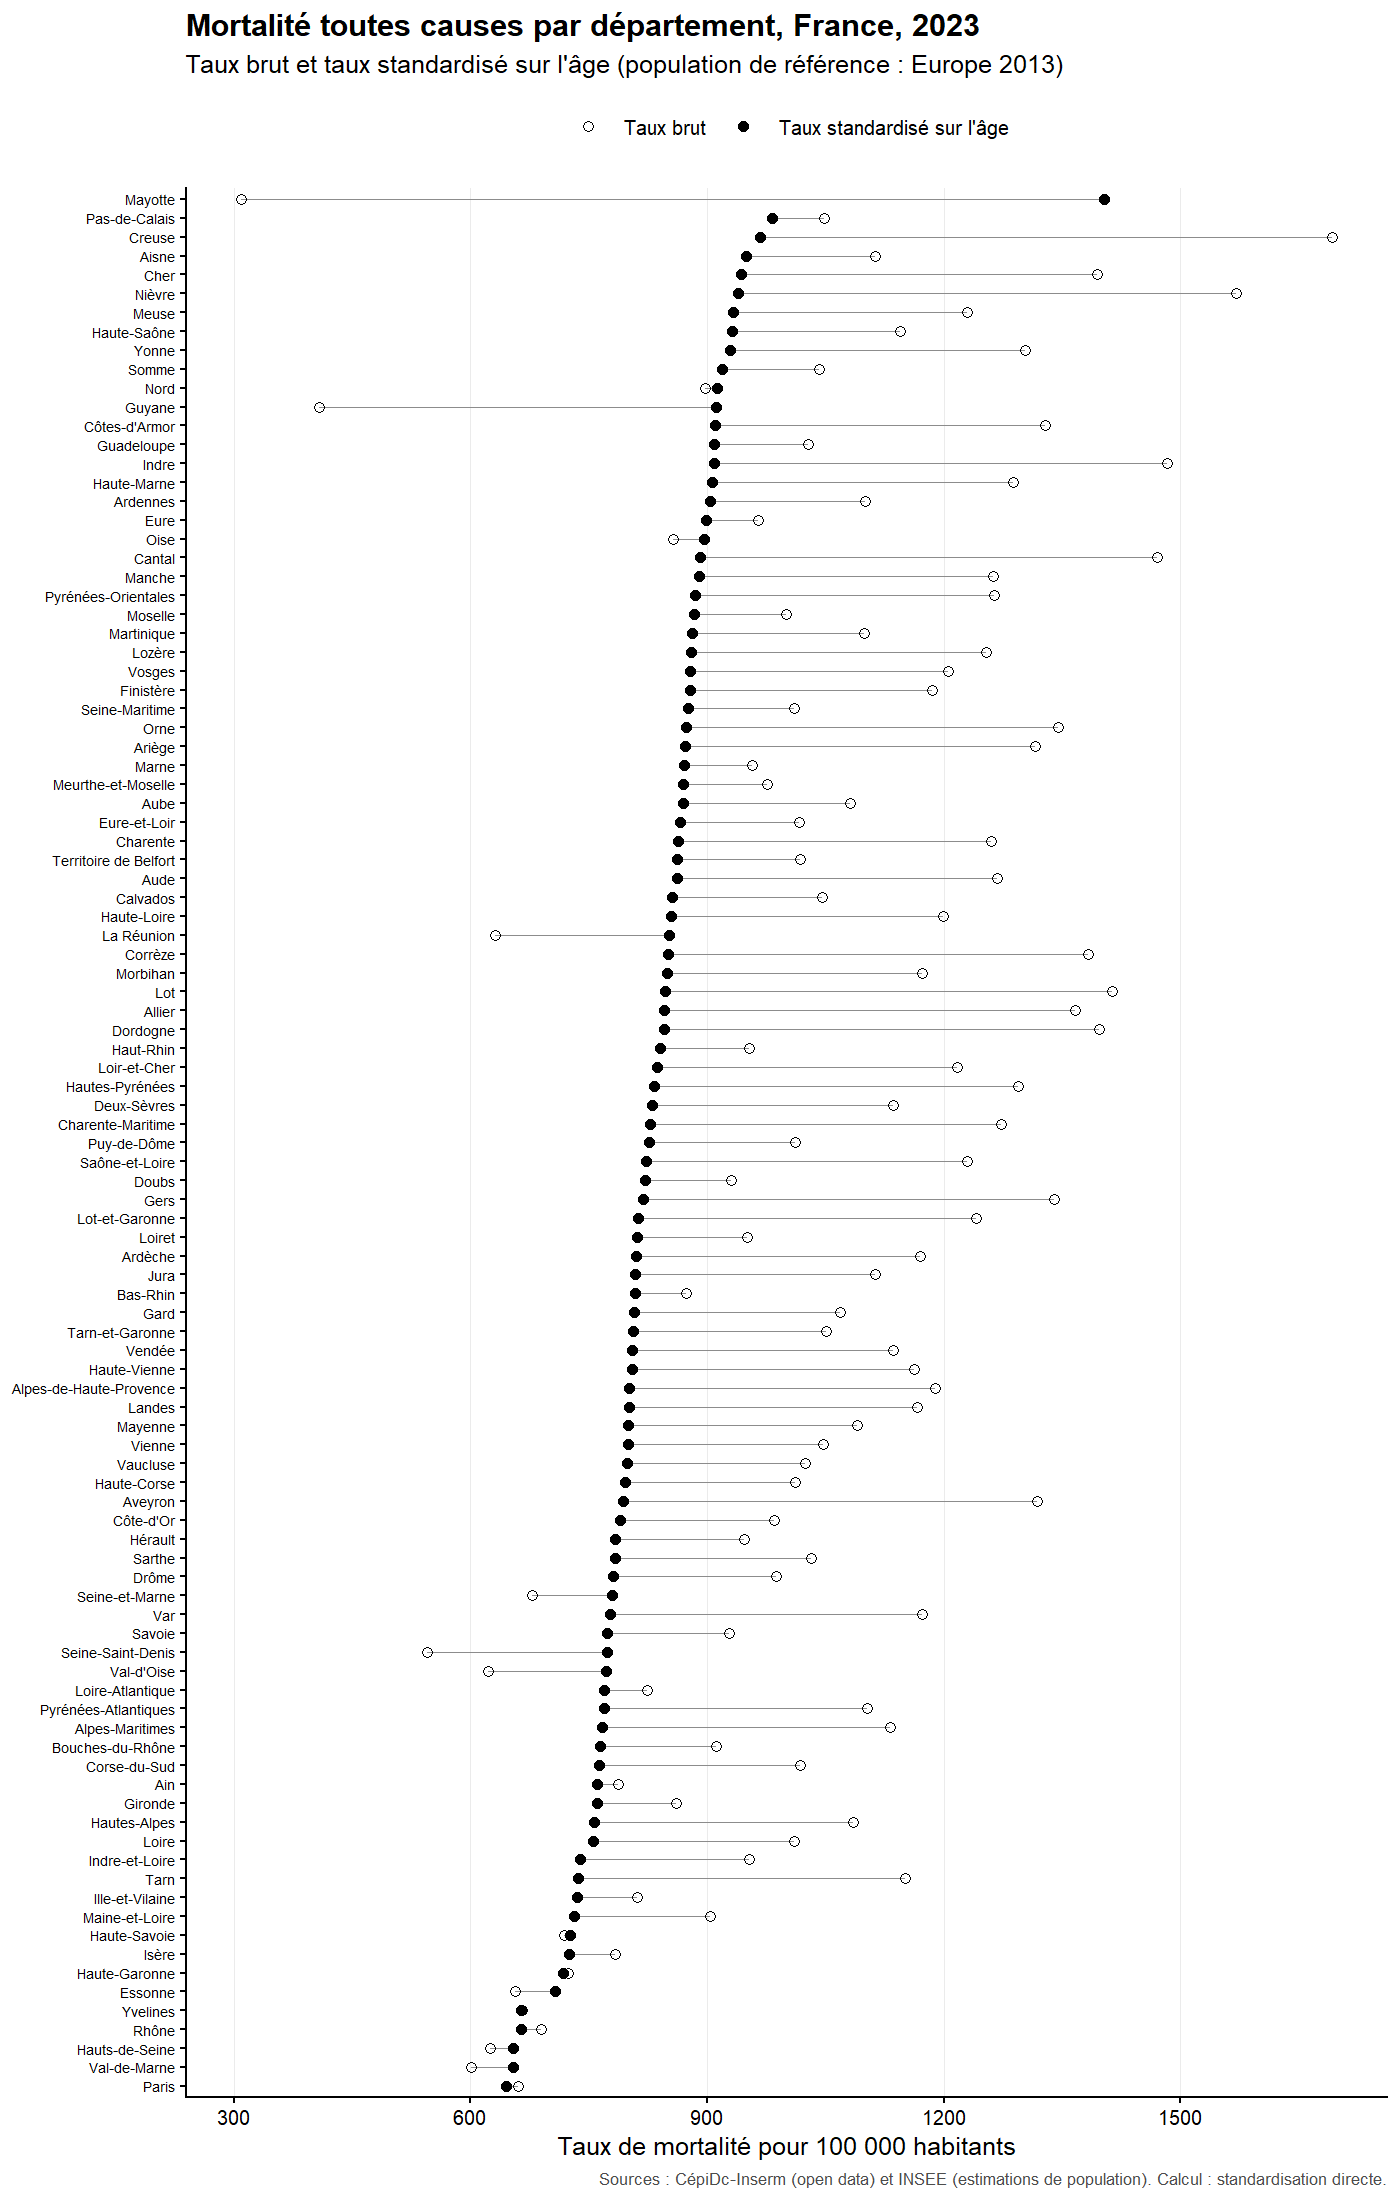
\includegraphics[height=0.92\textheight]{fig1_brut_vs_standardise.png}
\caption{Mortalité toutes causes par département, France, 2023. Pour chaque
département, le cercle vide donne le taux brut et le cercle plein le taux
standardisé sur l'âge (référence : population européenne 2013). Les départements
sont classés par taux standardisé. La longueur du segment mesure l'effet de la
structure par âge.}
\label{fig:dumbbell}
\end{figure}

\end{document}
